\chapter{Context and problematic}

\section{Crisis management domain}
\subsection{A definition?}
Defining the concept of crisis provides a hint of the challenges that lie within this domain.
Although the term is widely adopted in everyday language, it is paradoxically difficult to provide a precise and definitive scientific definition.
The term is used every day for both financial crashes and natural or humanitarian disasters.
Many researchers have tried to define this vague concept.
In 1994, \textcite{lagadecGESTIONCRISES1994} identified numerous attempts of definitions.
Taxonomies such as the one proposed by \textcite{rosenthalCrisisDecisionMakingNetherlands1986}, who, wishing a broader definition of "crisis", were interested in the different types of crises.
They then proposed the following taxonomy:

\begin{itemize}
    \item The "unimaginable" crisis, requiring that we really question the unthinkable (it does not appear very frequently).
    \item The "neglected" crisis.
    \item The "almost inevitable" crisis, in spite of a preventive action.
    \item The "compulsive" crisis, which results from inadequate management.
    \item The crisis sought by some, internal or external, actors.
    \item The crisis deeply desired by all parties.
\end{itemize}

In an almost similar way, \textcite{mitroffStructureManmadeOrganizational1988} proposed a classification of crises according to intrinsic characteristics.
The authors use a 2D matrix to classify the different types of events.
One of the components opposes the origin of the event (internal or external) while the other axis opposes the "social" or "technical" aspects.
For instance, company bankruptcies are located in the internal/technical quadrant, terrorist attacks in the external/human quadrant or natural disasters in the external/technical quadrant.
Brief definitions have also been proposed to define the term itself.
\textcite{hermannIssuesStudyInternational1972} proposed that "a crisis is a situation that threatens the essential goals of the decision-making units,
reduces the time available for decision making, and whose occurrence surprises those in charge".
More than a simple situation, \textcite{rosenthalCrisisDecisionMakingNetherlands1986} will prefer to insist on the notion of crucial decision making.
Thus, "A crisis is a serious threat affecting the basic structures or the fundamental values and norms of a social system,
which - in a situation of high pressure and high uncertainty - requires crucial decisions to be made."
But crises are also periods of uncertainty and disarray of organizations, where rules and processes are blurred.
\textcite{lagadecGESTIONCRISES1994} somewhat abandoned the notion of succinctness by proposing a more ambitious definition through a higher level viewpoint.
Thus a crisis is "a situation where multiple organizations, facing critical problems, subjected to strong external pressures, bitter internal tensions, are suddenly and for a long time projected on the front of the scene;
all this in a society of mass communication, that is to say "live", with the assurance of being on the front page of the radio news.

From the definitions given above, one can see the difficulty of defining the concept of crisis, as it is so diverse.
Crisis situations, although they appear to be a constant in our societies, seem to be out of reach due to the lack of regularity in the concept.
In the end, crises seem to be the demons living in the dark face of our societies.
Invisible and seemingly out of reach, we are only witnesses of their sudden and brutal irruptions in the visible phase of our world.
In fact, these irruptions invariably result in an eruption of chaos.
This metaphorical representation translates my personal vision of what a crisis is and the inherent complexity of the definition of this concept.
But while describing those "demons" seem an incredibly difficult endeavour, the irruptions themselves and their consequences possess common points.
Theses common points are the caracteristics discussed in the following.

\subsection{Some caracteristics of a crisis}
It now appears that a quantifiable and fixed definition of the concept of crisis is difficult to achieve.
However if the concept of crisis remains vague, the effects and consequences are real and quantifiable.
Victims, material damages, environmental destructions and other more or less reversible consequences are tangible and known by all.
A first characteristic that can be extracted from the previous definitions is the emergence of chaos that creates a brutal rupture.
Crises are thus to be distinguished from incidents, which are difficulties for which preventive measures allow to keep the situation under control.
In the absence of a definition, having an overview of the multi-dimensional consequences of crises is an important step in building an adequate representation of the concept.
The literature is rich in numerous efforts to inventory the manifestations of crises.
Many authors, sharing the observation that it is difficult to define the phenomenon, even propose to define crises based on their consequences.
Thus, for \textcite{milburnManagementCrisis1972}, only an event that meets certain criteria would be eligible for the title of crisis.
The characteristics they evoke are:

\begin{itemize}
    \item Threat to assets identified as essential by managers.
    \item Need for quick decisions.
    \item Relatively short time frame for response.
    \item Lack of emergency measures available, since it is an unforeseen situation.
    \item Need for innovation in solving the problem, due to the absence of a pre-existing system.
    \item Information overload.
    \item Ambiguity.
    \item Increase in the number and importance of requirements.
    \item Internal conflicts in the organization.
    \item Considerable fatigue.
\end{itemize}

This approach is discussed by \textcite{rosenthalCrisisDecisionMakingNetherlands1986}.
The latter put forward the problem of defining where to stop taking into account the effects of the crisis.
They consider that the previous list of limits does not sufficiently take into account all the facets of the crisis and in particular the opportunities that are created by such an event.
However, this first attempt to identify the characteristics of the crisis allows to identify certain characteristics.
In a similar approach, \textcite{finkCrisisManagementPlanning1986} define crises as situations that expose to risks.
Among the risks that identify we find the risk of:

\begin{itemize}
    \item Escalate;
    \item Attract significant media and administrative attention;
    \item Affect the normal operation of the company;
    \item Call into question the public image of the firm and its leaders;
    \item Reach the very foundations of the organization.
\end{itemize}

In the light of the two previous authors, \textcite{lagadecGESTIONCRISES1994} summarizes these caracteristics through three main caracteristics:

\begin{itemize}
    \item Surge: A crisis is a tsunami. Information, issues, external actors involved, media attention etc.
          Regular processing capacities are overwhelmed as everything is tenfold.
    \item Disruption: The universe in which the organisation/system was is falling appart. Allies are disengaging. New, unusual actors (and most ofen, unwanted) appear.
          An overall ambiguity is cast onto the system hit.
    \item Breakdown: The system is falling appart. The regularity is not anymore. All reference points both internal and external are disappearing.
          All the decisions are "no-win" for the organization.
\end{itemize}

These caracteristics are provided using a high level point of view and encapsulate a lot of concepts.
But they provide valuable information to create a big picture of what a crisis is.
In a different fashion, \textcite{fertierInterpretationAutomatiqueDonnees2018} proposed caracteristics that pave the way to a quantification of crisis events:

\begin{itemize}
    \item Geographic scope of the event.
    \item Duration (time between the first and last consequences, including replicas).
    \item The \emph{severity} of the event (minor/major). Scale established according to the number of victims and or material damage.
    \item The \emph{complexity} of the event, depending on the number of dimensions involved in the event, the number of layers and replicas of the crisis.
\end{itemize}

These criteria can be used as metrics to rank different events according to the impact they had.
Theses various caracteristics built over time highlight the diversity of consequences following a crisis event.
Caracterizing such events definitely benefits from a multidisciplinary approach, as different viewpoints lead to a different picture of the phenomenon of crisis.
The next paragraph presents the different terms used in this dissertation and provides the
semantic associated with them.

During nominal times, the \emph{population} lives in an \emph{environment} in which exist \emph{systems} composed of valuable \emph{assets} managed by \emph{organizations}.
Usually, when one studies a crisis, the point of view of an organization is taken.
The environment refers here to everything that is outside of the system or organization of interest.
The close environment can be composed of other assets part of other systems or organizations.
It can be other companies, other cities, other countries etc.
In the environment there are systems and their associated organizations that are impacted.
The part of the population that suffers from the event are considered as the \emph{victims} of the event.
Among all these systems, there is one of particular interest when a crisis happens: the crisis management system, which is in charge of the response to the event.
At crisis time, the organization in charge of crisis management creates a \emph{crisis cell}.
The United Nations Department of Humanitarian Affairs defines a crisis cell as "a facility officially designated for the direction and coordination of all actions in the response phase of a crisis".
The crisis cell is composed of \emph{operators} that gather, filter and share incoming information to the \emph{decision makers}.
The decision makers make \emph{decisions}, some of which are instructions to the \emph{response teams}.
A crisis has an effect on all the elements of the framework created above.
Using the created framework, one can see how the different characteristics mentioned above are positioned.

\subsubsection{The environment}
The first concept is the concept of environment.
The environment represents an area.
When an event hits, the environment can be splitted in two parts.
A part that is impacted by the event (the crisis environment) and the part that is not.
There are different kinds of crises, depending on the geographic scale of the event.
Some events can concern only a small industrial area, as in the case of water polution for instance, or have a worldwide scale, as in the case of the global pandemic that the world is facing at the time of writing this document.
Events with different scales involve actors accordingly.
A crisis can affect the environment in which systems and organizations exist in several ways.
But the main caracteristic effect is the sudden realization that the environment that decision makers were used to seems to have simply disappeared.
Infrastuctures, resources or actors that were supposed to be available are not anymore, or worse, their status are unknown to the decision makers.
Crises reshape the environment and consequently, the first steps taken once the organization realised that they lost control of the situation, is to figure out what this new environment looks like.
But not only the environment of the system is reshape, but the system itself is too.

\subsubsection{The system}
A system consists of: i) an organization in charge of the system and ii) issues that it considers important.
In fact, a crisis affects a system if and only if the system's stakes are threatened.
As an example, one can imagine the differences between a volcanic eruption near a city versus a volcanic eruption in a desert.
The former would be a dramatic event while the later would probably modify a few air traffic lanes.

Crises often result from the combination of different factors.
The organization in charge of the systems is supposed to protect the known vulnerabilities of the system and prepare for the unknown ones.
A crisis can emerge from a stressing event on one of those vulnerabilities.
To illustrate those interactions, \textcite{benabenCollaborativeSystemsCrisis2014} propose a framework which illustrates the relation between the different concepts Figure~\ref{context:fred-framework}.
The consequences are, according to the previous authors, the result of an event on risks (which we call here vulnerabilities).
These risks are in their turn the result of dangers on stakes.

\begin{figure}
    \centering
    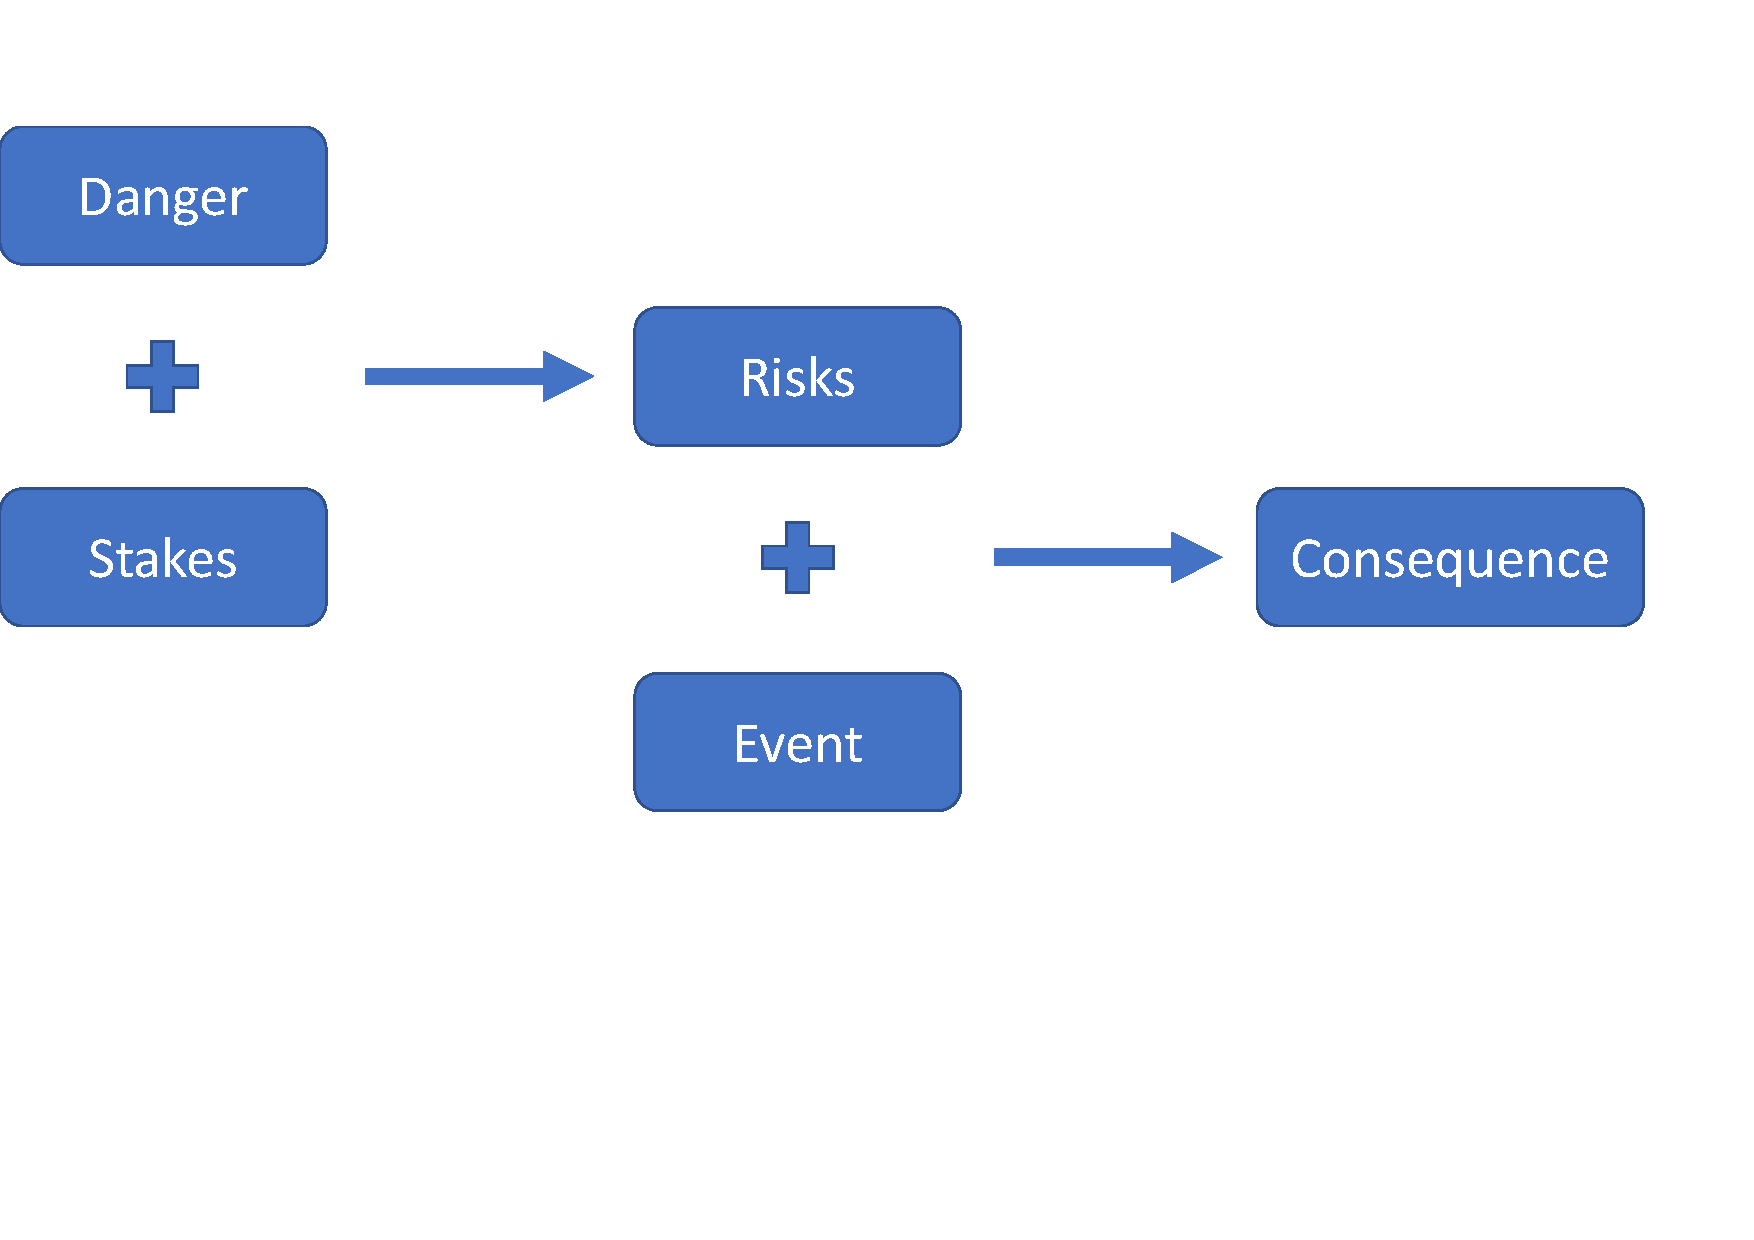
\includegraphics[width=\textwidth]{figures/fred-consequences-framework.pdf}
    \caption{Crisis causality chain from \textcite{benabenCollaborativeSystemsCrisis2014}}
    \label{context:fred-framework}
\end{figure}

Each consequence can in turn become a danger or an event that endangers the system.
\textcite{fertierInterpretationAutomatiqueDonnees2018} puts forward this phenomenon through what it names "the cascade effect".
The crisis is self-feeding with the dynamism explained before and drags the system in its fall.
The best known industrial example is undoubtedly the Chernobyl nuclear disaster.
The cascade effect also joins the "surge" evoked by \textcite{lagadecGESTIONCRISES1994}, which is based on numerous testimonies of people who were involved in the crisis management.

In the end, a complete disruption of the system occurs.
Normal operation is no longer possible. The existing processes are no longer valid.
The historical partners are no longer available while unusual actors appear.

The consequence of this disruption is the increase in complexity of the operations.
Additional precautions are required for each decision and intervention that follows.
Every action that was once trivial becomes uncertain.
Most of the usual signals have disappeared and the remaining ones are ambiguous.
At the same time, the information requirements for each decision explode.
The intact parts of the system freeze into inaction.

\subsubsection{The organization}
The organization is the group of individuals that compose and manage a system.
The employees of a company, the first responders, all of them compose the organization with respect to a hierarchy between the different members of the organization.

The organization during the crisis is in charge of responding to the event.
It must protect the system and especially the assets.
In this sense, the organization can prioritize the value of the assets.

The activation of the response depends on how long it takes the organization to realize that the event is there.
There may be a lag time between the first effect of the crisis and the activation of the response.
By the time the response is activated, the crisis has already impacted a significant part of the system and its state is therefore altered.
This change in the state of the system plunges the organization into uncertainty and doubt.
The system is no longer in a known state.
The situational awareness has changed and there is an urgent need to re-establish a coherent vision for further response operations.
The situational awareness of an organization and its impact on the response are further developed in chapter 2 of this manuscript.
Then begins the reclamation of information for the organization.
From this point on, every decision made is crucial, to protect the stakes.
But with the loss of knowledge about the state of the system, every decision comes with a lot of uncertainty.

To reduce uncertainty, the organization will seek to know the state of the system.
It therefore requires reports on all aspects of the system.
The organization is successively drowned under two consecutive waves.
The first one concerns the feedback of information on the different dysfunctions and limitations that have appeared.
The second wave is about reporting on the state of the environment and the system as a result of the need to regain visibility for decision making.
This reporting may be partially automatic for automated systems and if the sensors have not been influenced by the crisis.
For emergency services (911, firemen), this feedback is essentially done via the response units deployed and the calls of the impacted people.
Similarly, external services (meteorological, specialized...) can also provide external data to help the organization make decisions.
However, the organization is rarely prepared to handle so much information and the organization becomes overwhelmed.

In addition to this, the initial information feedback is scattered and therefore ambiguous.
The context in which each piece of information fits is absent or limited.
The situation faced by the organization can be illustrated with a puzzle.
However, we do not know the final outcome of the puzzle and the pieces are provided to us one after the other, in no particular order.
We are also forced to place the pieces of the puzzle (i.e. make decisions) without having the following pieces.
Under these conditions, it is only possible to complete the puzzle when enough pieces are provided.
To imagine the psychological consequences of such a way of completing the puzzle makes it obvious why we don't do puzzles in this way.

In addition to these internal difficulties, there is also the external pressure.
The event inevitably attracts the attention of regulators, higher authorities and the media.
The organization, sometimes unknown until then, finds itself under the spotlight.
Its past is scrutinized, looking for previous mistakes that may have led (or not) to the current event.
Its leaders and their decisions are dissected and the inconsistencies are highlighted as soon as possible in order to feed the headlines.
Thus, in addition to the physical impact of the crisis, the trust and the image of the organization is also weakened.

\subsubsection{The decision makers}
The decision makers are the people with responsibility in the organization.
Most of the organizations are hierarchical.
In fact, there is also a hierarchy of decision makers.
The decisions of some individuals thus take precedence over those made by their subordinates.
Of course, at the time of a crisis, this phenomenon increases tenfold, adding to the already existing confusion.

Moreover, all the decisions look like "no-win" for the organization.
The problems pile up without them having time to solve any of them.
The knowledge of the whole they are in charge of has suddenly disappeared as well as the assurance it gave them.
Their perception is distorted, as much as their assumptions, and each new decision is a disappointment that slowly leads them to realize that there are no more good decisions, only fewer bad ones.
Of course, all this is done in a hurry, created by the influx of requests and reports.
Decision making is further complicated by the fact that the usual processes and safeguards they used to rely on potentially no longer exist or have become irrelevant.
Improvisation and innovation, once feared, is now required with the realization that inaction will be as, if not more, costly than action.
The stress on the organization is hitting decision makers hard.
Under the urgency, stress and fatigue, every decision becomes a battle to be fought in this war that the crisis has created.

This first part of the chapter presents my vision of the crisis and what it implies.
This vision will drive the manuscript, including the structure of the different concepts affected by a crisis - the environment, the system, the organization and the decision makers.
The reminder of this section develops how organizations deal with these situations.

\subsection{Crisis Management}
Crises are not a question of "if" but of "when".
This inevitability implies an upstream reflection on the part of organizations and a consideration of this problem within the systems.
These practices are called crisis management.

Wikipedia defines crisis management as "the set of organizational modes, techniques and means that allow an organization to prevent,
prepare for and respond with the occurrence of a crisis, and then to draw lessons from the event to improve procedures and structures
with a forward-looking vision" (Wikipedia, 2021).
This definition perfectly highlights two main characteristics of crisis management.
First, crisis management is more a broad spectrum methodological toolbox than a set of recipes to be applied in case of an event.
Secondly, it takes into account the different temporal phases of the crisis.
In the following, we detail these two aspects.

\subsubsection{The crisis management cycle}
The crisis management literature identifies four major phases.
These phases are most often represented in the form of a cycle.
The cycle illustrates the inevitability that we mentioned earlier. (put the references).
The 4 phases are :

\begin{itemize}
    \item Prevention : phase aiming at preventing the appearance or reducing the effect of an emergency situation.
          This phase consists of identifying potential hazards that threaten system vulnerabilities and appropriate measures.
    \item Preparedness: Measures that facilitate the response to the disaster. It involves ensuring that resources are available and deployable, that response personnel are trained, and that the potentially impacted organization is psychologically prepared.
    \item Response: corresponds to the activation of measures "is engaged from the beginning of a major event, to take cognizance of the situation, go to resources, make decisions
          and follow up on actions in progress".
    \item Recovery: Phases that follow the response to the crisis. It corresponds to the repair/reconstruction of the parts of the system impacted by the event.
          This stage is often accompanied by an analysis of the risks associated with the repairs, in order to avoid creating a replica of the crisis.
\end{itemize}

In this cycle, only one transition between two phases is clear: the one between preparation and response.
This transition occurs when the organization acknowledges the event and goes into crisis management.
The other transitions correspond more to a duration where two phases coexist.
The prevention phase, however, leads to some debate.
\textcite{benabenCollaborativeSystemsCrisis2014} argue that the prevention phase is, in fact, common to the whole cycle.
Even during the response and the recovery, the organization observes prevention measures to prevent cascading effects.
If prevention is common to the whole cycle, the cycle can be simplified with only three phases in crisis management: the preparation (before the event), the response (during the event), the recovery (after the event).

Also, it is possible to see beyond the cyclic representation.
Today's world is complex, tense and deeply interconnected. % Reference?
As a result, large organizations or countries possess a large surface vulnerable to potential disruptive events.
Then, instability and crisis management somehow become the norm.
Small and large incidents trigger responses from the organization.
However, these events are concurrent to each other and each one is at a specific phase of the cycle.
Consequently, looking at the global picture, these organizations are dealing with multiple crises at the same time.
Similarly, large crisis situations are often not dealt at the global level directly.
A local firefighters station will not deal with a hurricane by itself for example, but rather will take care of smaller, local events that are the direct consequences of the hurricane.
Here again, the hurricane triggers the response phase in the cycle, but one could zoom into this phase and see that there are in fact many smaller and concurrent cycles happening at the same time.
The cycle representation of crisis management does not account to the scale nor the complexity of events, but it is a good enough abstraction to represent the different times in an event.

\subsubsection{Stakes in Crisis Management}
As said before, crises threaten stakes of a system.
Crisis management is the tool used to oppose crises and composes one of the systems present during a crisis situation.
This system has its own stakes during an event.
As a result, the crisis management system faces problems that vary depending on the phase of crisis management the system is in at any given time.
Numerous authors from the information systems domain have studied these different issues and identified stakes.

During the response phase, \textcite[.~12--18]{fertierInterpretationAutomatiqueDonnees2018} identifies 5 stakes for the organization:

\begin{itemize}
    \item The collaboration between internal and external stakeholders.
    \item The situational awareness~\footnote{Chapter 2 of this manuscript is devoted to the meaning of "situational awareness" for an information system. For this reason we will not go into further detail here.} associated with the environement and the system.
    \item The data obtained during the event from different sources.
    \item The information acquired from the previous data.
    \item The system in charge of data and information processing.
\end{itemize}

\textcite{batardIntegrerContributionsCitoyennes2021} also identifies two of the previous stakes as the overarching stakes in responding to a crisis situation:

\begin{itemize}
    \item The knowledge of the situation
    \item Coordination of the various actors
\end{itemize}

From these two main stakes, the author then proposes four axes to protect those.

First, the management of the multiplicity of data sources.
Organizations in charge of crisis management are already used to taking into account several data sources.
Feedback from the field from the staff allocated to the response as well as phone calls from victims or witnesses of the event are commonly used.
However, new sources are emerging such as the Internet of Things and the various sensors that can provide interesting records regarding certain events.
The rapid and global development of social media is also a potentially interesting source of data \textcite{meierStrengtheningHumanitarianInformation2013}.
The opportunities offered by this data source are detailed in section 1.2.3.

Secondly, the automatic interpretation of these data to extract relevant information.
This information is then delivered in an adapted way to the decision makers \textcite{luokkalaDevelopingInformationSystems2014,vandewalleImprovingSituationAwareness2016}.

Thirdly, the management of information systems adapted to the crisis management context.
This information system is supported by an IT system, whose role is to facilitate the response.
This facilitation is enabled by delegating some of the tasks necessary to i) restore situational awareness and ii) coordinate actors to the IT system \textcite{benabenManagementCollaborativeBehavior2015}.

Fourth, the information system and the computer system must be adaptable.
This strong constraint results from the nature of crisis situations.
A crisis management system must therefore be able to detect changes in the situation and react to them in an adapted manner \textcite{barthe-delanoeEventdrivenAgilityInteroperability2014,charlesModelDefineAssess2010}.

These previous analyses, strongly oriented towards information systems, highlight key stakes during crisis management.

\begin{enumerate}
    \item An understanding of the current situation and state of the environement.
    \item The coordination of the actors, that needs to be fluid and orchestrated accordingly to the event.
    \item A system for collecting and organizing the available data.
    \item A system for managing the information extracted from the data, adapted to the context of crisis management and its users needs.
\end{enumerate}

This analysis allows us to succinctly summarize the needs of the actors during crisis management.
Thus, the organization responsible for crisis management must first restore its knowledge of the situation using the data available to it.
Secondly, it must manage the information obtained from these data in order to best coordinate its response with its internal and external actors.

\subsection{Tools for crisis management}
The previous section identified 2 main stackes from the information system point of view: the coordination of the actors and the restoration, then management, of the situational awareness.
The protection of these stakes by the system is of the utmost importance to allow an adequate response.
Tools and practives have been developed to help organizations in charge of crisis response to address those issues.

\subsubsection{Organizational modes}
The organization of the response is one of the components of the preparation phase.
During this phase, the different future actors of the response agree on the roles of each and their responsibilities during the future event.
For instance, in the response phase, the system dealing with the response uses a hierarchical organization, layered with crisis cells.
A crisis cell is a facility officially designated for the direction and coordination of all actions in the response phase of a crisis.
They bring together the decision makers of the organization who implement and direct the various actors to respond to the crisis.
Thus, the crisis units must have a high-level vision of the event, but also be close to the actors of the response they are managing.
Large-scale crises (mobilizing many actors or a large territory, for example) will undoubtedly lead to the creation of a hierarchy of crisis units.
While the "low-level" crisis units orchestrate the response, a "higher-level" crisis unit is responsible for transmitting information between the "low-level" crisis units and coordinating their responses.
In France, this hierarchy is composed of 5 levels:

\begin{itemize}
    \item European
    \item National
    \item Zonal
    \item Departemental
    \item County
\end{itemize}

Each of the crisis cells set up has its own specificities, depending on the actors who compose it.
However, all are constrained by the same need for collaboration \textcite{benabenAIFrameworkMetamodel2020,comfortCrisisManagementHindsight2007} and information \textcite{comfortCrisisManagementHindsight2007,endsleyTheorySituationAwareness1995}.
It is precisely the role of the information system to manage and exchange situation-specific information between the different actors.

\subsubsection{Techniques and Methods}
The organization mentioned above is only effective if the actors coordinate their actions.
This coordination requires the communication of information available to the different actors.
The organization's information system is in charge of this aspect.

Wikipedia \textcite{InformationSystem2021} proposes the following definition of information system.
"An information system (IS) is a formal, sociotechnical, organizational system designed to collect, process, store, and distribute information.
From a sociotechnical perspective, information systems are composed of four components: task, people, structure (or roles), and technology.
Information systems can be defined as an integration of components for collection, storage and processing of data of which the data is used
to provide information, contribute to knowledge as well as digital products that facilitate decision making."
This definition mixes the definition provided by \textcite{oharaManagingThreeLevels1999,piccoliInformationSystemsManagers2019,zwassInformationSystemDefinition}.
Thus, the organization's information system is the cornerstone of information management within the organization.
It can be digitalized or not, depending on the needs and practices of the organization, as it reflects how the information is processed in the physical organization.
The information system is an abstract concept that encompasses many aspects of the organization.
The development and maintenance of the information system is performed during the preparation phase.
During this phase, hardware and software must be deployed, tested and used for training to ensure smooth operation during the response.
The hardware aspects are outside the scope of this manuscript, which is mainly interested in the software and social part of the information system Figure~\ref{context:information-system}.

\begin{figure}
    \centering
    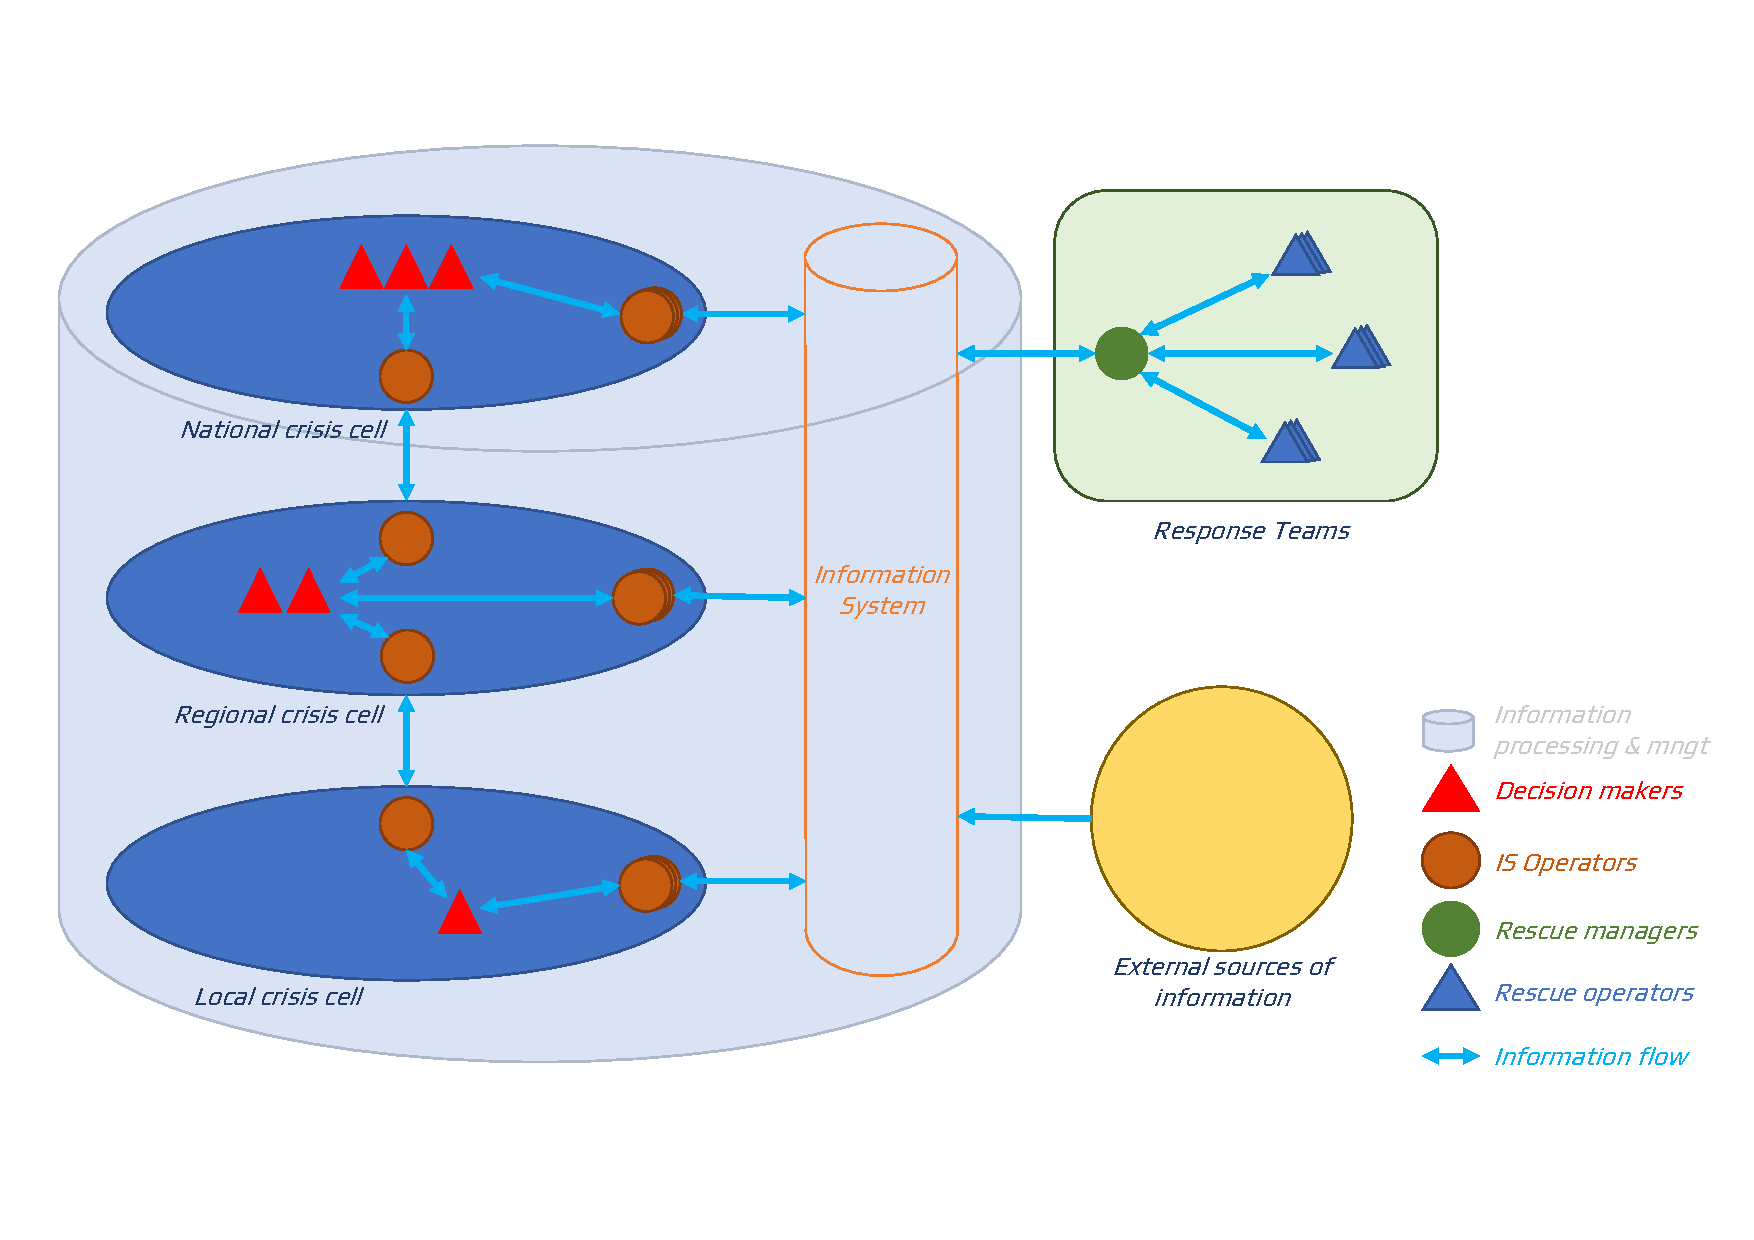
\includegraphics[width=\textwidth]{figures/information-system.pdf}
    \caption{Representation of a crisis information systems and its interaction with the different members of the organization}
    \label{context:information-system}
\end{figure}

The role of an information system is, according to the definition, to collect, process, store and distribute information.
The information system is thus fed by data sources.
In France, \textcite{morelEtudePriseDecision2010} indicate that fire department services mainly receive their data from three sources:

\begin{itemize}
    \item The calls that victims make from emergency numbers.
    \item The crews deployed to respond to the crisis.
    \item Other organizations involved in crisis management.
\end{itemize}

The rest of the manuscript assumes that these data are common in most of the emergency services activated during the response to an event.

The previous part detailed the way crisis cells are organized in crisis response, and the hierarchy built to scale decision making with the size of the event.
Each actor of this hierarchy comes with its own, internal information system.
However, to enable the coordination between all the different actors, information has to flow between each of them.
Yet, two challenges arise.
First, the actors have to share a common vocabulary in order to communicate.
Secondly, the information system has to be designed to allow communication.

The distribution of information is often hampered by misunderstandings between the different actors.
The latter often have different skills, responsibilities and roles.
Each actor therefore builds his own vocabulary, his own terminology to designate the elements in his field of action.
If this facilitates daily operations, during an event, it complicates the collaboration and communication between the actors \textcite{opachMapbasedInterfacesCommon2020}.
The preparation phase is therefore an opportunity to identify the actors who will potentially be brought to collaborate during an event, and to bring them together so that they are familiar with each other's culture.

Common format and representations of the information between all the actors is needed to build a common understanding of the situation.
From a technical point of view, the different actors can decide to set up a "Commission Operational Picture (COP)".
According to \textcite{UnitNIMSCommunications}, a COP is "A representation that is established and maintained by collecting, collating, synthesizing and disseminating information among the different participants.
It allows the different actors to have access to the same information regarding the availability and location of resources and the status of different requests for assistance".
Thils representation is often cartographic, allowing the geographic component of an information to be easily represented.
Geographic information is also information that is equivocal among all actors.
The COP is therefore a tool that allows to initiate and build a dialogue between the different actors of the response.
It is also the visible face of the information system.
The COP benefits from all the advantages that the rest of the information system provides.
The COP can be automatically fed with the above mentioned data.
Thanks to this data, the information system can then produce useful information for the decision makers, and make it available automatically on the COP \textcite{fertierInterpretationAutomatiqueDonnees2018}.
One of the problems currently faced by COPs is their inability to communicate with each other most of the time, due to mutually exclusive software, which does not offer the possibility of dialogues between them \textcite{opachMapbasedInterfacesCommon2020}.

\begin{figure}[h]
    \centering
    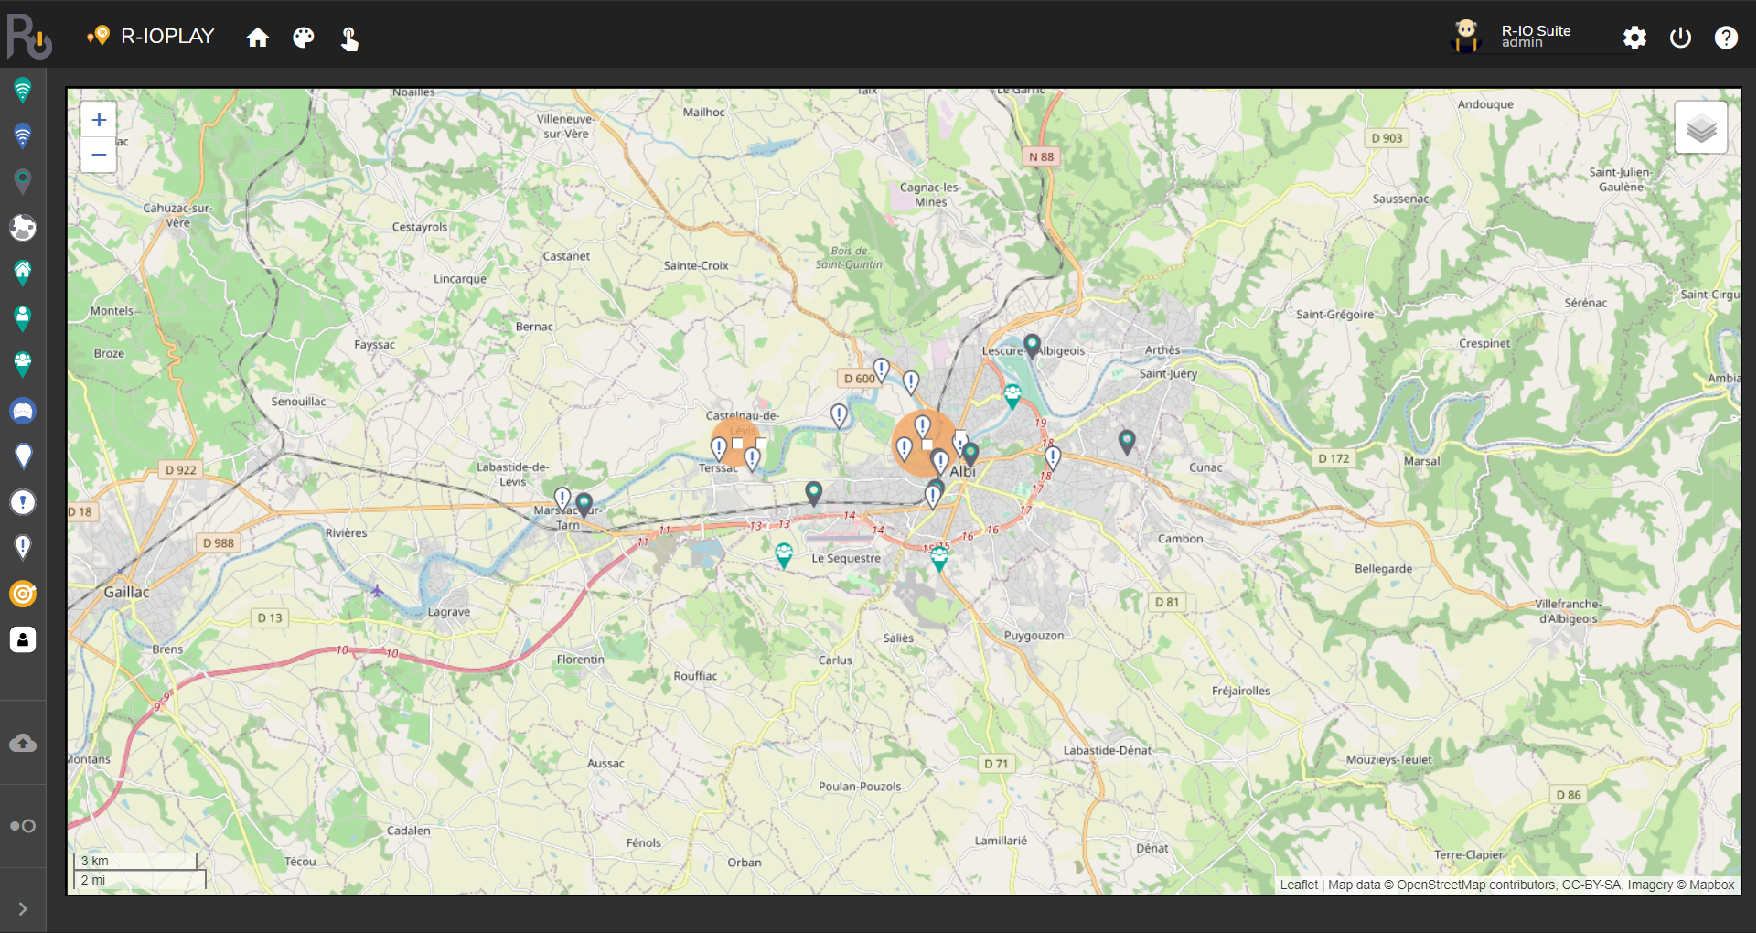
\includegraphics[width=\textwidth]{figures/rio.pdf}
    \caption{Cartographic display of the R-IOSuite software in a flood scenario in France\protect\footnotemark}
    \label{context:cop}
\end{figure}
\footnotetext{https://research-gi.mines-albi.fr/display/RIOSUITE/Welcome}

Finally, the COP is an asset for building and maintaining adequate and shared situational awareness among all actors.
As we saw earlier, the restitution of situational awareness is one of the challenges of crisis management, as is the coordination between the different actors.
The COP is an asset because it is a tool that allows both issues to be addressed simultaneously.

Crisis management is a challenging domain.
By nature, crises events are uncertain and hard to define.
Yet, patterns emerged from this uncertainty especially when it comes to information management.
Regardless of the event, decision makers are in dire need of information about the impact of the event on their system and organization.
Tools and methodologies have then been developped to assist the decision makers from the different organizations in coordinating and understanding the situation.
Research and development  around digital tools to support information management takes place in the crisis informatic domain \textcite{palenCrisisInformaticsHumancentered2020}.
One of those tools is the Common Operational Picture.
The COP is a map shared between the different actors, with common, but also specific information, displayed.
This representation is the visual face of a common information system used by all the actors.
However, the COP comes with its one challenge, as each individual information system has to be able to share information with the common one.
Also, the different actors have to agree on common representations and terminologies that will be used by the COP.

\section{Social media}
\subsection{What are social media?}
In the previous chapter, we identified the informational needs of decision makers during crisis events.
At the same time, and somewhat paradoxically, our societies have never had so many means and platforms to exchange information.
Among these platforms, social media have recently appeared.
Social media are Internet platforms that appeared during the Web 2.0 era.
The term Web 2.0 was developed between 2003 and 2007, by T. O'Reilly.
This terminology was initially born to revive the economy of the Web after the explosion of the dot.com bubble formed during the development of Web 1.0 consisting mainly of web portals.
Web 2.0 reflects the development of the community web and is organized around platforms that allow their users to connect with each other in order to co-create and share content \textcite{oreillyWhatWebDesign2007b}.
Social media fits into this definition.
\textcite{kaplanUsersWorldUnite2010} identify 6 types of social media: blogs and micro-blogs (e.g. Twitter), social networking sites (e.g. Facebook), collaborative projects (e.g. Wikipedia), content communities (e.g. Youtube), virtual social worlds (e.g. Second Life) and virtual game worlds (e.g. World of Warcraft)

Social media are now essential websites and platforms that have up to one billion users in the case of Facebook.
Like the crises we mentioned earlier, it is difficult to grasp their full dimensions.
These platforms, often global, connect users from all over the world, forming a true digital double of our societies.
The multitude of cultures, communities, languages and codes that co-exist in a single place has no equivalent in the history of humanity.
The disproportionate size of these platforms is accompanied by opportunities and threats.
Social media are indeed a great gateway to the world, allowing to connect with an incredible number of people around the globe.
It is also an efficient way to share information and exchange with other users, through many formats.
If the majority of social media users are consumers of content, a significant portion of them also create content \textcite{fuchsSocialMediaCritical2021}.
The creation of content on these platforms is thus their cornerstone, so much so that some of these platforms do not hesitate to pay their users who contribute, thus making a new profession emerge: content creator.

But with this opportunity to unite humanity in a few hubs on the Internet, comes many challenges.
Spreading false information, harassment campaigns against individuals or state disinformation, feeding political disengagement or addictions are some of the problems associated with social media.
If all these problems are not exclusive to these platforms, their dimensions and dynamics amplify them greatly.
The rest of this section draws the reader's attention to two components of interest in understanding social media, namely what is a social network and what is viral information.
Other keys to understanding may be of interest as well, but for the sake of brevity these will be the only two mentioned in this manuscript.

\subsection{Some social media caracteristics}
\subsubsection{On the Social Network}
Most people live in a community.
Family, friends, neighbors, colleagues, all of these circles form an individual's social network.
The social network is an integral part of one's life.
Some researchers have looked into the question of what the social network of different individuals could look like.
Obviously, a network is a graph, and this question has a strong link with mathematics.

It is therefore not surprising that the first interesting results come from a mathematician.
By being interested in random networks, \textcite{erdosEvolutionRandomGraphs1960} discovers that each node of the network is on average separated from any other node by six intermediate nodes.
More surprisingly, this result is little affected by the size of the network.
It was not until a few years later that these results, which had until then been essentially theoretical, found a concrete application in the social sciences.
\textcite{milgramSmallWorldProblem1967}, verified the validity of the previous results within a population of individuals.
Each node then becomes an individual and the edges are the relationships between the different individuals.
Their results obtained in this physical experiment validated the theoretical results on random networks.
This property is now known as the "six degrees of freedom".

\textcite{wattsCollectiveDynamicsSmallworld1998} sought to deepen the understanding of the six degrees of freedom and discovered on this occasion the structure in small worlds of social networks.
So if people meet each other by chance as in Paul Erdös' model, the social network itself is rather composed of small communities, with many links between individuals
and very few links between communities.
This model is called "small world network", because, contrary to intuition, the majority of individuals in the network are connected by very few intermediaries, regardless of the distance between them or the community to which they belong.

Similarly, \textcite{barabasiEmergenceScalingRandom1999} deepens Paul Erdös' random model by discovering another property of social networks.
Indeed, the random model predicts that the distribution of the number of friends among individuals must follow, by construction, a normal distribution.
However, this is not what they discover experimentally.
The distribution of the number of friends among individuals follows a power law.
This property thus forms a scale invariant network, where individuals connect preferentially to the most influential nodes.

In reality, both models have their properties verified.
We can therefore consider, as a first approximation, that the two models coexist.
Therefore, a social network can be described through three main properties:

\begin{itemize}
    \item Each individual can be linked with only a few intermediaries (6 on average), whatever the size of the network
    \item The network is structured in communities that are very connected to each other.
    \item The communities are connected by a few individuals who act as hubs.
\end{itemize}

These properties are illustrated on Figure~\ref{context:social-network}.

\begin{figure}
    \centering
    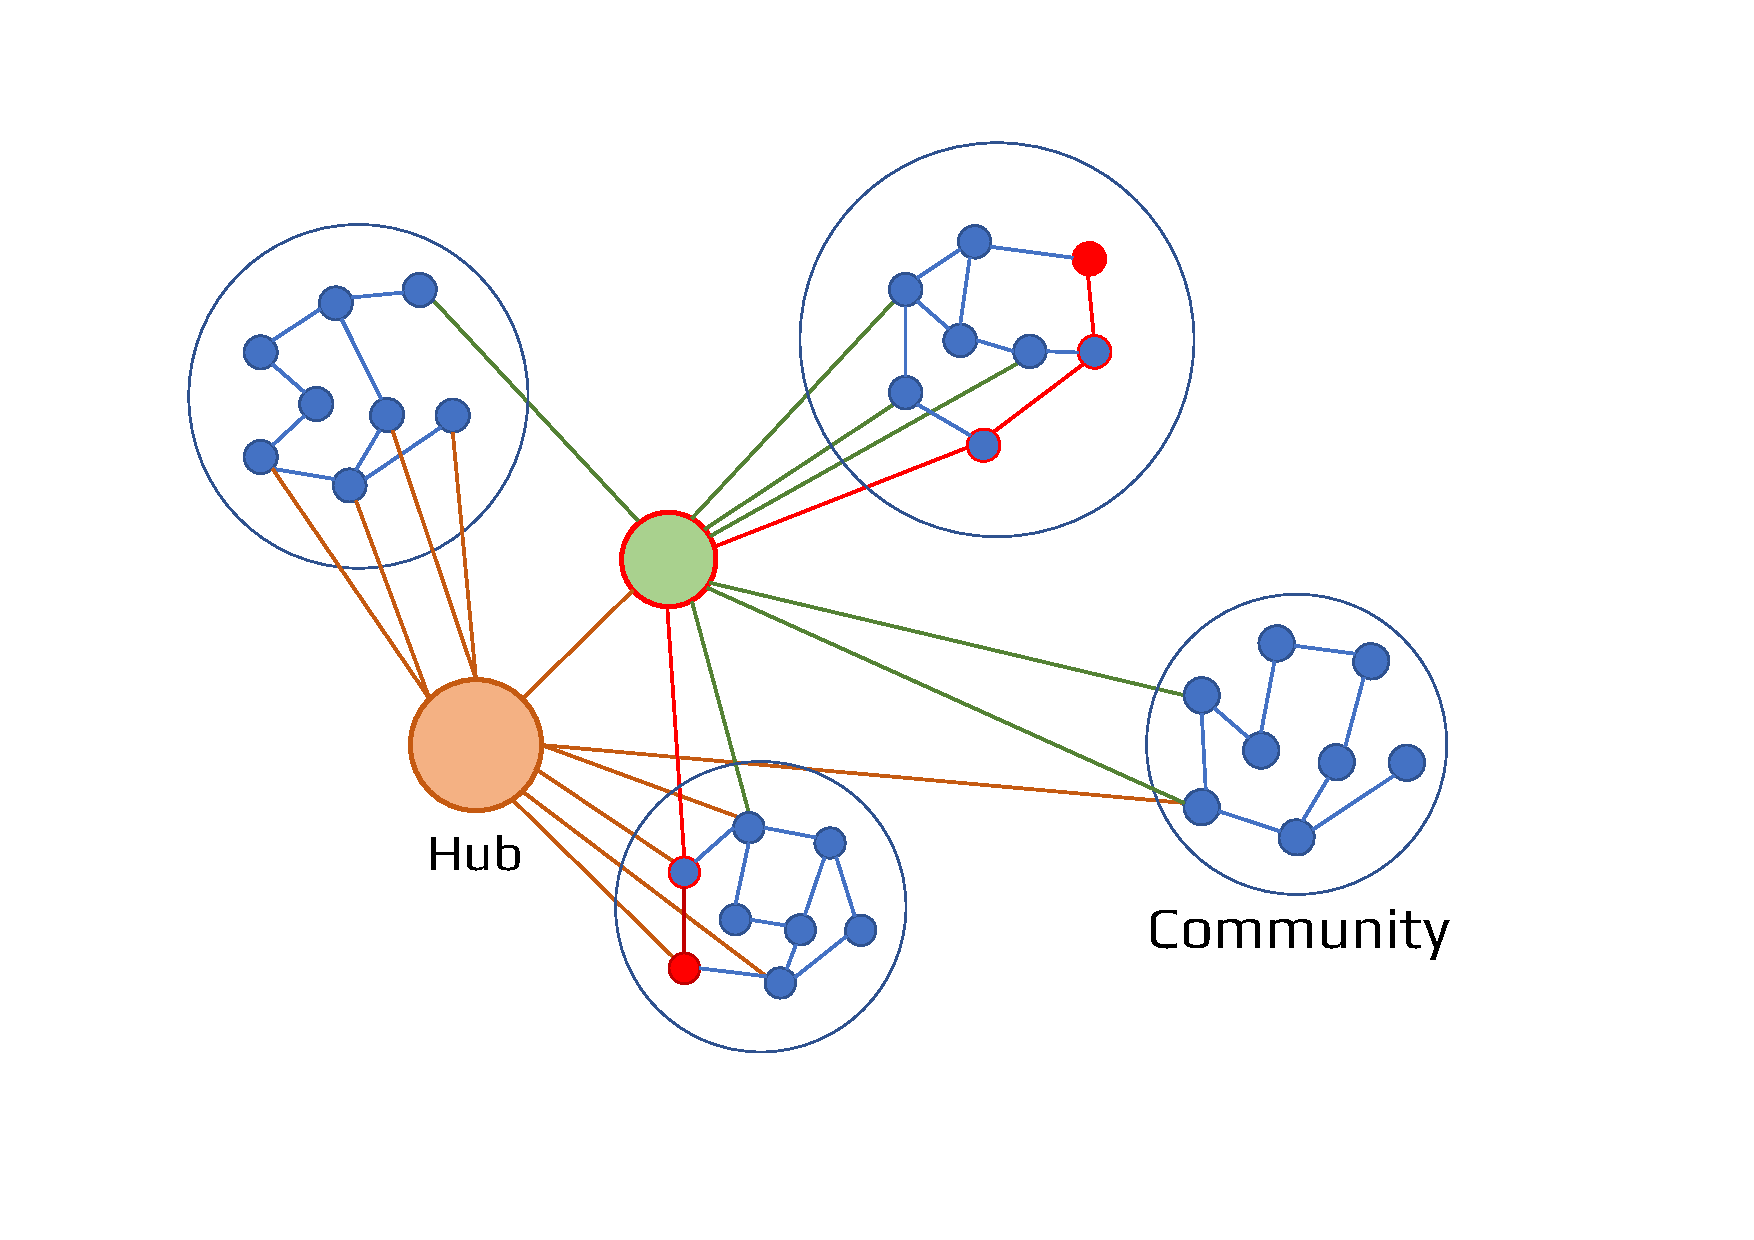
\includegraphics[width=\textwidth]{figures/network.pdf}
    \caption{Illustration of the combination of both social network models from \textcite{wattsCollectiveDynamicsSmallworld1998} and \textcite{barabasiEmergenceScalingRandom1999}.}
    \label{context:social-network}
\end{figure}

These properties are valid whether the social network is "real" or virtual - many of the experiments in the previous publications were obtained by studying social media.
Thus, social media can be seen as a multitude of communities, linked together by hubs (influencers).
Having the structure of social networks in mind allows us to better understand the propagation of information within a social network.
This brings us to the next section, and a topic familiar to all social media users: viral information.

\subsubsection{On Virality}
The propagation of information, true or false, within a community is experienced daily by everyone.
However, this characteristic of information sharing is exacerbated in the case of social media for two reasons.
First, social media brings together a large number of users in one place.
Second, they provide their users with a number of tools that aim to make information sharing much easier.
By construction, social media put information and content sharing at the center of their strategy.
However, in a social network, each user can easily reach any user in very few intermediaries, regardless of the size of the network.
Moreover, information can quickly reach a very large number of users if it is shared through network hubs.

This speed of dissemination is thus unusual, as are the results that such propagation can generate.
Research teams are therefore interested in understanding what viral information is and how this virality is characterized.
By studying chains of information propagation, they identify that the phenomenon of virality is quite rare.
Large content cascades are the exception, not the rule.
99\% of posts are reposted less than 10 times, while cascades of more than 1,000 reposts are created by 0.001\% of the posts.
Viral content is therefore rare, but when it goes, it is seen by a large number of users.

Recently, the notion of virality on social media has been widely associated with the term "fake news".
Fake news are a concern that grew with social media platforms themselves.
Particularly, in the 2016 US election context, the involvement of Russia in the process through disinformation campaigns~\footnote{https://www.judiciary.senate.gov/meetings/extremist-content-and-russian-disinformation-online-working-with-tech-to-find-solutions}
brought even more attention to that problematic.
\textcite{lazerScienceFakeNews2018} define fake news as a "fabricated information that mimics news media content in form but not in organizational process or intent".
The authors warn about the stakes and threats posed by fake news on our societies and call for more efforts to understand these dynamics, which are still largely misunderstood.
Also, viral content cascades depend on the veracity of the content they propagate.
Thus, false information spreads faster, to more people, for longer with an essentially vertical structure (friends of friends relay the information).
On the contrary, real information spreads more slowly, to fewer people, with slower kinetics and an essentially horizontal structure (the information is essentially shared by the sender's followers).
Deriving from the previous results, \textcite{vosoughiRumorGaugePredicting2017} built a system that assesses the veracity of one piece of information, based on the way this information is propagated.
Their method achieves a classification score of 75~\% using only this simple feature.

Finally, the understanding of the propagation of information on social media remains largely marginal.
The call to link more independent research to the platforms of \textcite{lazerScienceFakeNews2018} remains largely anecdotal, effectively hindering progress in this field.
In the following section, we explore, in light of the few elements presented so far on social media, the different opportunities for crisis management.

\subsection{Opportunities and threat posed by social media for crisis management}
The previous sections highlight the digital double role of the social media society.
These platforms offer a point of view never seen before

Important events have long had an imprint on the Internet.
In the aftermath of the September 11 attacks in New York, web pages for exchanging information about people were created \textcite{palenCitizenCommunicationsCrisis2007}.
The relationship between crisis events and social media is now well established.
The case of the ditching of the U.S. Airways Flight 1549 on the Hudson River in New York City in January 2009 is often used as an example of the impact that social media can have in important situations.
The information of the ditching had indeed been relayed on social media before all the traditional media \textcite{murthyTwitter2018}.
Other studies have highlighted the reaction of social media during crisis situations, as in the case of tornadoes in the United States \textcite{justinei.blanfordTweetingTornadoes2014}.

However, crisis management requires data and information to be able to achieve its objectives.
Social media appear as a potential source of information for emergency services \textcite{tapiaSeekingTrustworthyTweet2011}.
Moreover, where phone calls were the only link with the population, this digital twin of society offers a real time overview of the conversations and feelings of the people who are affected by the event.
These platforms thus make available a wide variety of data, which can help emergency services.
As content creation platforms, users can use the wide range of tools at their disposal to share information about the ongoing event.
Texts, photos and videos can help crisis decision makers to better understand the event, even in places where they have no resources deployed.
Social media can also bring back information that may have been missed by other actors within the organization.
Finally, users of these platforms not directly impacted may decide to help the victims.
These volunteers, digital or not, could be mobilized to assist the emergency teams deployed on the scene of the event \textcite{batardIntegrerContributionsCitoyennes2021}.

The full potential of social media is yet to be discovered.
However, these platforms come with challenges.
As mentioned in the previous section, fake news is a current problem with social media \textcite{lazerScienceFakeNews2018,vosoughiSpreadTrueFalse2018,oshikawaSurveyNaturalLanguage2018}.
This phenomenon is also mentioned in crisis management and attracts some interest from the scientific community \textcite{starbirdExaminingAlternativeMedia2017,sellMisinformationUSEbola2020}.
However, while misinformation and the sharing of false information is something we see on social media in crisis situations, it is not necessarily indicative of their uses alone.
\textcite{bubendorffConstructionDisseminationInformation2021} indeed highlights the small amount of information involved and the self-correcting effect of the crowd, which ultimately reduces the impact of false information.
Despite this, emergency services remain cautious about the use of information from social media.
By focusing on the use of social media by the latter, \textcite{tapiaGoodEnoughGood2014} also highlights their fears, which the authors believe are unfounded.
Because one of the main challenges of social media still lies in their relative novelty and the lack of understanding of their universe.

Social media are Internet platforms that provide content creation tools to their users, allowing them to generate and share data.
Altogether, Twitter, Facebook, Reddit, Instagram, Youtube and many others, have billions of users worlwide who share their everyday life, creations and feelings with their communities.
These digital twins of the society are ressourceful and possess valuable information for crisis management.
However, the dynamic of these platforms remain hard to understand for individuals and, in light of the recent controversies that have sprung, many are questioning their utility to ease crisis response.

\section{Natural Language Processing}
\subsection{On Natural Language Processing}
"Computational linguistics, also known as natural language processing (NLP), is the subfield of computer science concerned with using computational techniques to learn, understand, and produce human language content." \textcite{hirschbergAdvancesNaturalLanguage2015}."
As "learn, understand, and produce human language content" is a broad objective, the field is subdivided into major tasks :
Some of these tasks are:

\begin{itemize}
    \item Language recognition
    \item Machine translation
    \item Sentiment analysis
    \item Question answering
    \item Text summarization
\end{itemize}
The rest of this section presents the concepts and terminologies used in NLP.

NLP is concerned with textual data.
There is no lack of such data, as this format is used extensively to share information on the Internet (wikis, emails, messages, etc.).
To a computer, text is a sequence of ASCII or UTF-8 entities, called \emph{characters} in the format of bytes (or eight bits).
A set of textual data is called a \emph{dataset} or a \emph{corpus} (both terms will be interchanged thoughout this manuscript).
Corpora are most of the time composed of two parts: the \emph{metadata} and the text itself.
Metadata provide the context in which the data exists (e.g. a timestamp, recipient, receiver etc.)
The text in the corpus can be \emph{tidy} or \emph{raw} and in the latter case, will require a step of \emph{preprocessing}.
The characters in the sequence are grouped in units called \emph{tokens} during a process called \emph{tokenization}.
Tokenization depends on the language.
Western languages can split tokens using white-spaces or punctuation, but this way of splitting text can't be used for Japanase (that do not contain any space) or Turkish (as an agglomerative language) for instance.
Contiguous multitokens are called \emph{spans} and are used to represent high order tokens for specific tasks such as \emph{chunking} and \emph{named entity recognition}.
For instance, in the sentence "Bob scored a goal", we might want to extract the noun "Bob" and the verb "scored".
Named entity recognition aims at a similar objective, but with \emph{named entities}, a string mention of a real-world concept such as locations, organizations, persons etc.
All the unique tokens form the \emph{vocabulary} or \emph{lexicon} of the corpus and individuals are called \emph{types}.
These types can be either \emph{content words} or \emph{stopwords}, the latter being mostly used for grammatical purposes rather than for conveing information.
Also, words have one or more meanings.
The \emph{senses} are all the meanings of a word.
The WordNet project intends to catalog the senses of the words in the English language \parencite{millerWordNetLexicalDatabase1995}.
As of writing (2021/07/19), WordNet contains more than 150.000 words and their senses.

NLP is mainly achieved through 3 main approaches \parencite{hirschbergAdvancesNaturalLanguage2015}:

\begin{itemize}
    \item Rule-based approach : rules are written to match certain tokens or groups of tokens
    \item The statistics-based approach : a statistical model is trained to recognize word distributions and find them in new entries.
    \item The deep neural network approach.
\end{itemize}

The revival of deep neural networks, driven by the explosion of available data volume and computational power, has found a place in NLP.
The ability of these models to build fine abstract components of the data patterns has allowed significant progress in NLP.
These advances are especially visible on the semantic part of the text.
Where once one relied mainly on the structure and syntax of the text, deep neural networks now allow us to add an important semantic component to the processing.

\subsection{NLP and Social Media: A natural match}
The section dedicated to social media highlighted how much these platforms provide tools to their users to create content.
This results in a significant amount of data created by the content creator for their communities.  % Add numbers here
These platforms embedded data type such as text, images and videos.
Also, all the content possess metadata that provide context at processing time and in turn, leverage a lot of opportunities.
A large portion of this data are textual data.
This amount of data can hardly be processed by human agents alone.
Thus, the need for an automatic processing method, such as NLP.

However, most NLP methods and tools are developed using textual data from news articles and books mostly written in english.
Social media data rarely look like this type of data, as they are more informal, conversational.
Messages on social media often use emoticons, non-standard spelling and abbreviations, making tokenization even more challenging.
As an example, tweets (messages publised on Twitter) can contain @handles, \#hashtags https:\/\/urls and smileys :-) that need to be processed.
Thus, the medium, or even the platform, can require a specific tokenizer.
The lack of grammar also complicates syntactic analyses.
Absence of punctuation also makes detection of sentence boundaries challenging.

Social media are also a very noisy source of data.
Posts from users are mostly direct reports of their current thoughts.
Hence the use of "status" to mention social media posts, as users share with their community their instant feelings.
Messages are also more subjective compored to news articles, where the objectivity of the information matters.

Lot of reseach have been done to explore the possibilities of social media, in a wide variety of domains.
highlight in their fourth chapter different use case in several domains:

\begin{itemize}
    \item healthcare: tracking of depression, PTSD, schizophrenia, pharmaceutical side-effects or flu season
    \item financial: computation of socio-economic indicators based on the sentiment of the general population, tracking of financial communities advices
    \item political: predicting voting intentions
    \item media monitoring: tracking of news worldwide
    \item security and defense: pre identification of possible threats, tracking of incident reports
    \item etc.
\end{itemize}

Natural language processing provides valuable tools to those who want to process textual data.
More importantly, it allows to process automatically large amount of data and to make sense of it.
On the other hand, social media are platforms that contain a large amounts of textual data posted by millions of users worldwide.
Processing this amount of data requires automatic processing.
Thus NLP and social are two domains that naturally fit together.

\section{At the crossing paths of the domains}
The previous sections described three domains: i) the crisis domain, ii) the social media domain and iii) the NLP domain.
Also, as presented earlier, these domains intersect.
Crisis management requires information to operate.
Social media produce data, which can be converted into information.
NLP tools provide ways to extract information from textual data.
Thus, there is an intersection between the different areas (Figure~\ref{context:venn-diagram-domains}).

\begin{figure}
    \centering
    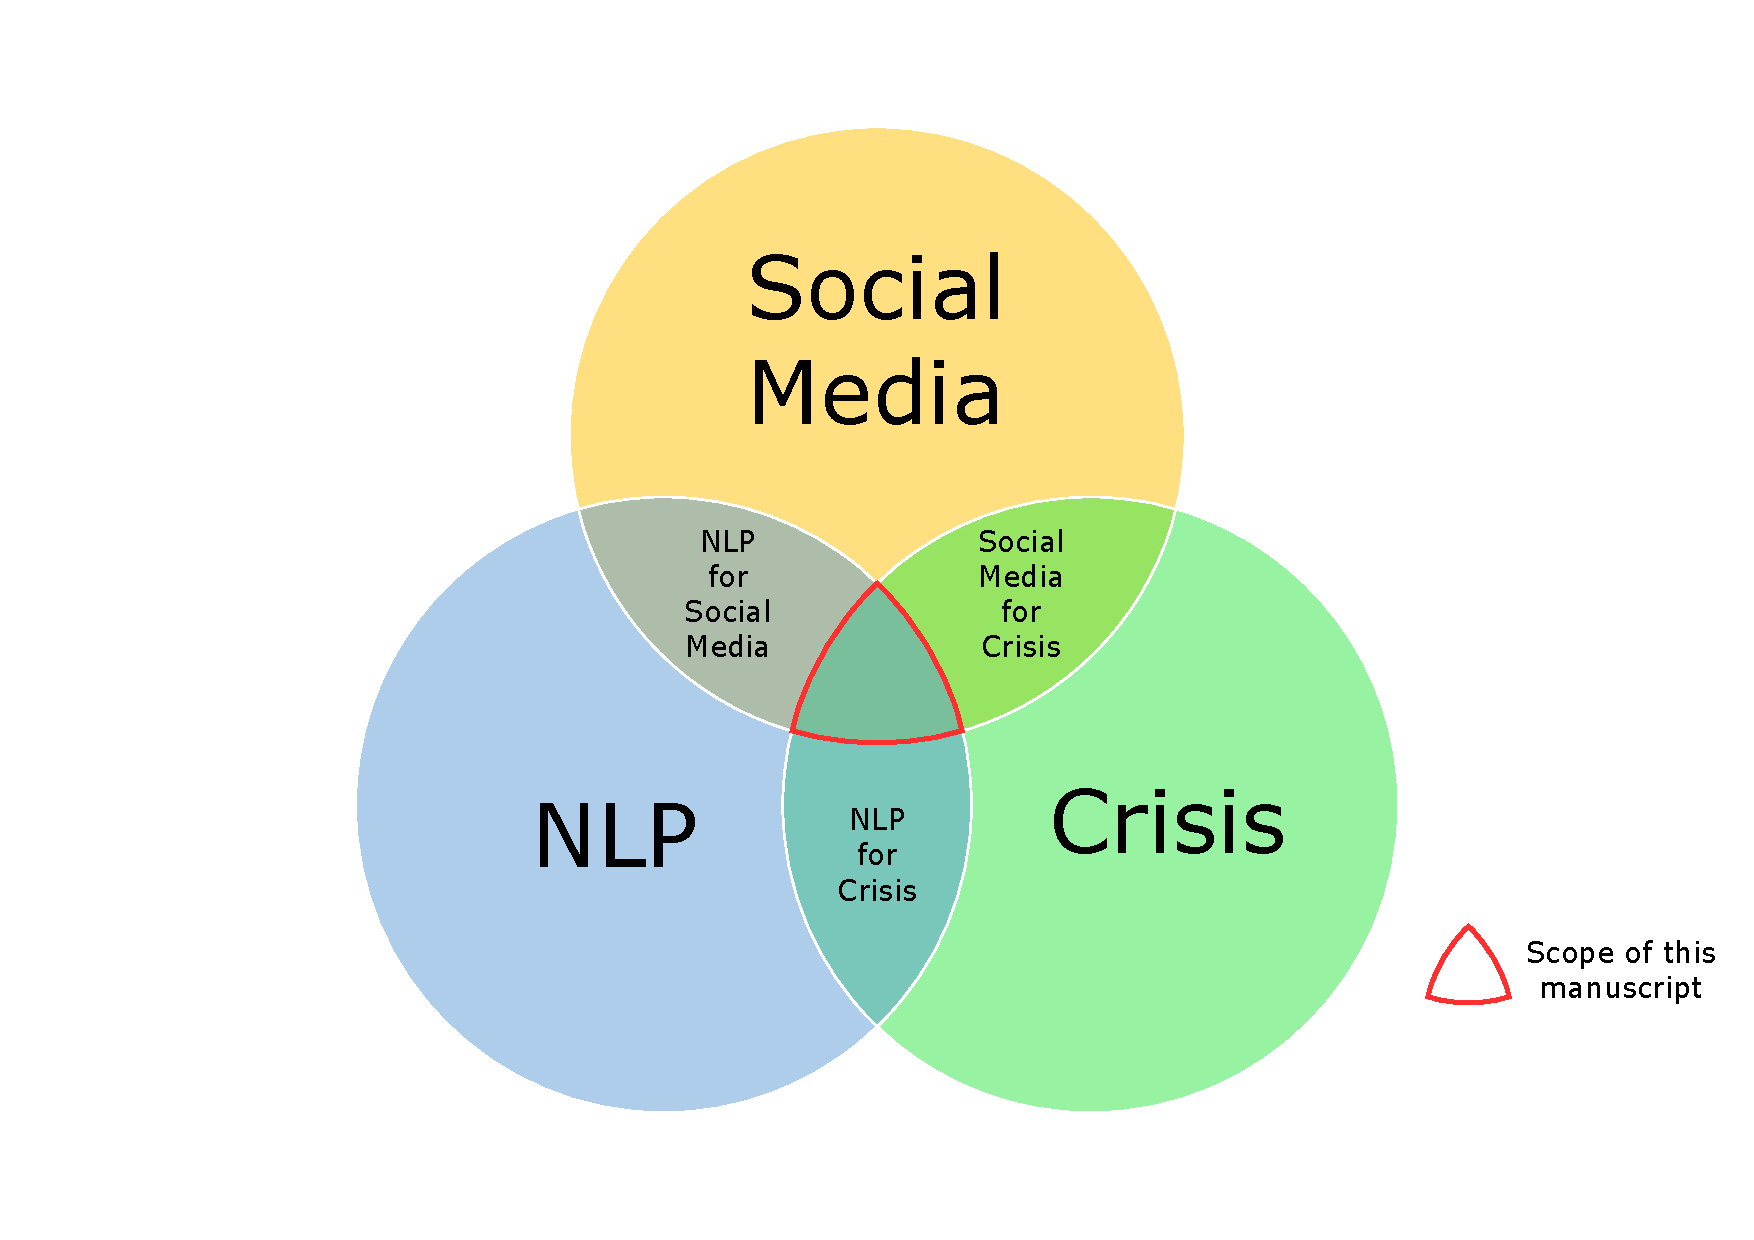
\includegraphics[width=\textwidth]{figures/venn-diagram-domains.pdf}
    \caption{Intersection between the domains of Social Media, Crisis Management et Natural Language Processing and the positioning of the research presented in this manuscript.}
    \label{context:venn-diagram-domains}
\end{figure}

\textcite{palenCitizenCommunicationsCrisis2007} highlighted in 2007 the role of information and communication technologies (ICT) in crisis response.
A few years later, social media were considered as an opportunity in crisis management \textcite{viewegMicrobloggingTwoNatural2010}.
This work started the social media branch of crisis informatic \parencite{palenCrisisInformaticsHumancentered2020}.
NLP was then used to automatically retrieve information from the flow of social media data \textcite{vermaNaturalLanguageProcessing2011,carageaClassifyingTextMessages2011}.
This allowed to scale the analysis to the high volume of content that social media have to offer.
Most of the early work was spent in ways to automatically identify crisis related text messages.
Since then, many efforts have been added to explore other opportunities, such as images.
Variations on different types of crises, on NLP techniques, and features used to represent the data were developed and used.
\textcite{imranUsingAISocial2020} identifies several remaining challenges in the domain of social media in crisis informatic:

\begin{itemize}
    \item Crisis event detection
    \item Eyewitness detection
    \item Situational awareness
    \item Actionable information gathering
    \item Damage assessment
    \item Crisis communication
    \item Understanding public reaction
    \item Information veracity
\end{itemize}

All these challenges aim at extracting information from social media media.
They necessarily involve artificial intelligence to identify at scale the mentioned information.
However, as mentioned earlier, social media data are subjectives, fuzzy and prone to rumors.
At the same time, the outcome of NLP models is never 100\% accurate.
Thus, uncertainty is the norm among the information extracted from social media data.
Also, all these information, once created, need to be stored, managed and distributed, to provide
Thus, the following problematic:

\begin{center}
    \fbox{
        \begin{minipage}{0.75\textwidth}
            \centering
            \emph{Main problematic:}

            How to design an information system able to automatically manage and deliver relevant information extracted from social media data?
        \end{minipage}
    }
\end{center}

This main problematic is then decomposed into three sub-problematics.

\subsection{Consecutives challenges to the main problematic}
Three consecutives challenges to the main problematic arise.
Firstly, the objective is to identify

\begin{center}
    \fbox{
        \begin{minipage}{0.75\textwidth}
            \centering
            \emph{Research question 1:}

            What information that can be obtained from social media is relevant to the decisiom makers in crisis response?
        \end{minipage}
    }
\end{center}

Secondly, once relevant information has been identified, one needs to collect the data needed and
extract the information wanted. Thus, the second research question:

\begin{center}
    \fbox{
        \begin{minipage}{0.75\textwidth}
            \centering
            \emph{Research question 2:}

            How can the information expected by the decision makers be automatically retrieved, given the context of the crisis response?
        \end{minipage}
    }
\end{center}

Thirdly, extracting information is not enough.
This information needs to be managed, to deliver further value, and delivered.
Leading to the third research question:

\begin{center}
    \fbox{
        \begin{minipage}{0.75\textwidth}
            \centering
            \emph{Research question 3:}

            How is this information organised to deliver the value expected by decision makers?
        \end{minipage}
    }
\end{center}

\subsection{The MACIV project}
The MACIV project (Management of Citizens and Volunteers: the social media contribution in crisis situations)
was an opportunity to bring together multiple actors from different institutions around the problematic
of adoption of social media in crisis response.
The objective of the project was to understand the opportunity offered by volunteers in crisis management, especially in the social media space.
This project, funded by the Agence National de la Recherche (ANR), was composed of both
scientific actors — Télécom ParisTech, IMT Mines Albi and —,
institutional actors — Direction Générale de la Sécurité Civile et de la Gestion des Crises, Préfecture de Police de Paris, Service Départemental d'Incendie et de Secours du Var — and
associatives actors — the VISOV (Volontaires Internationaux en Soutien Opérationel Virtuel) association.
This collaboration was illustrated through three different, physical, exercices.

Along this project which took place in France, a significant part of the work presented in this dissertation was fed through a year long in the USA.
This visiting provided opportunities to meet several actors of the American  emergency services that
provided valuable insights that fueled the results presented later in this document.

\section{Structure of the document}
The purpose of this manuscript is to advance the issue of improving situational awareness and collaboration between actors during the response to a crisis event, which was one of the issues identified in the crisis management section.
Thus, adopting the point of view of decision makers, and in the scope of the information system, the main problematic is:

\emph{How to design an information system able to automatically manage and deliver relevant information extracted from social media data?}

The scope and consecutives research questions of this main problematic are illustrated in Figure~\ref{context:big-picture}.

\begin{landscape}
    \begin{figure}
        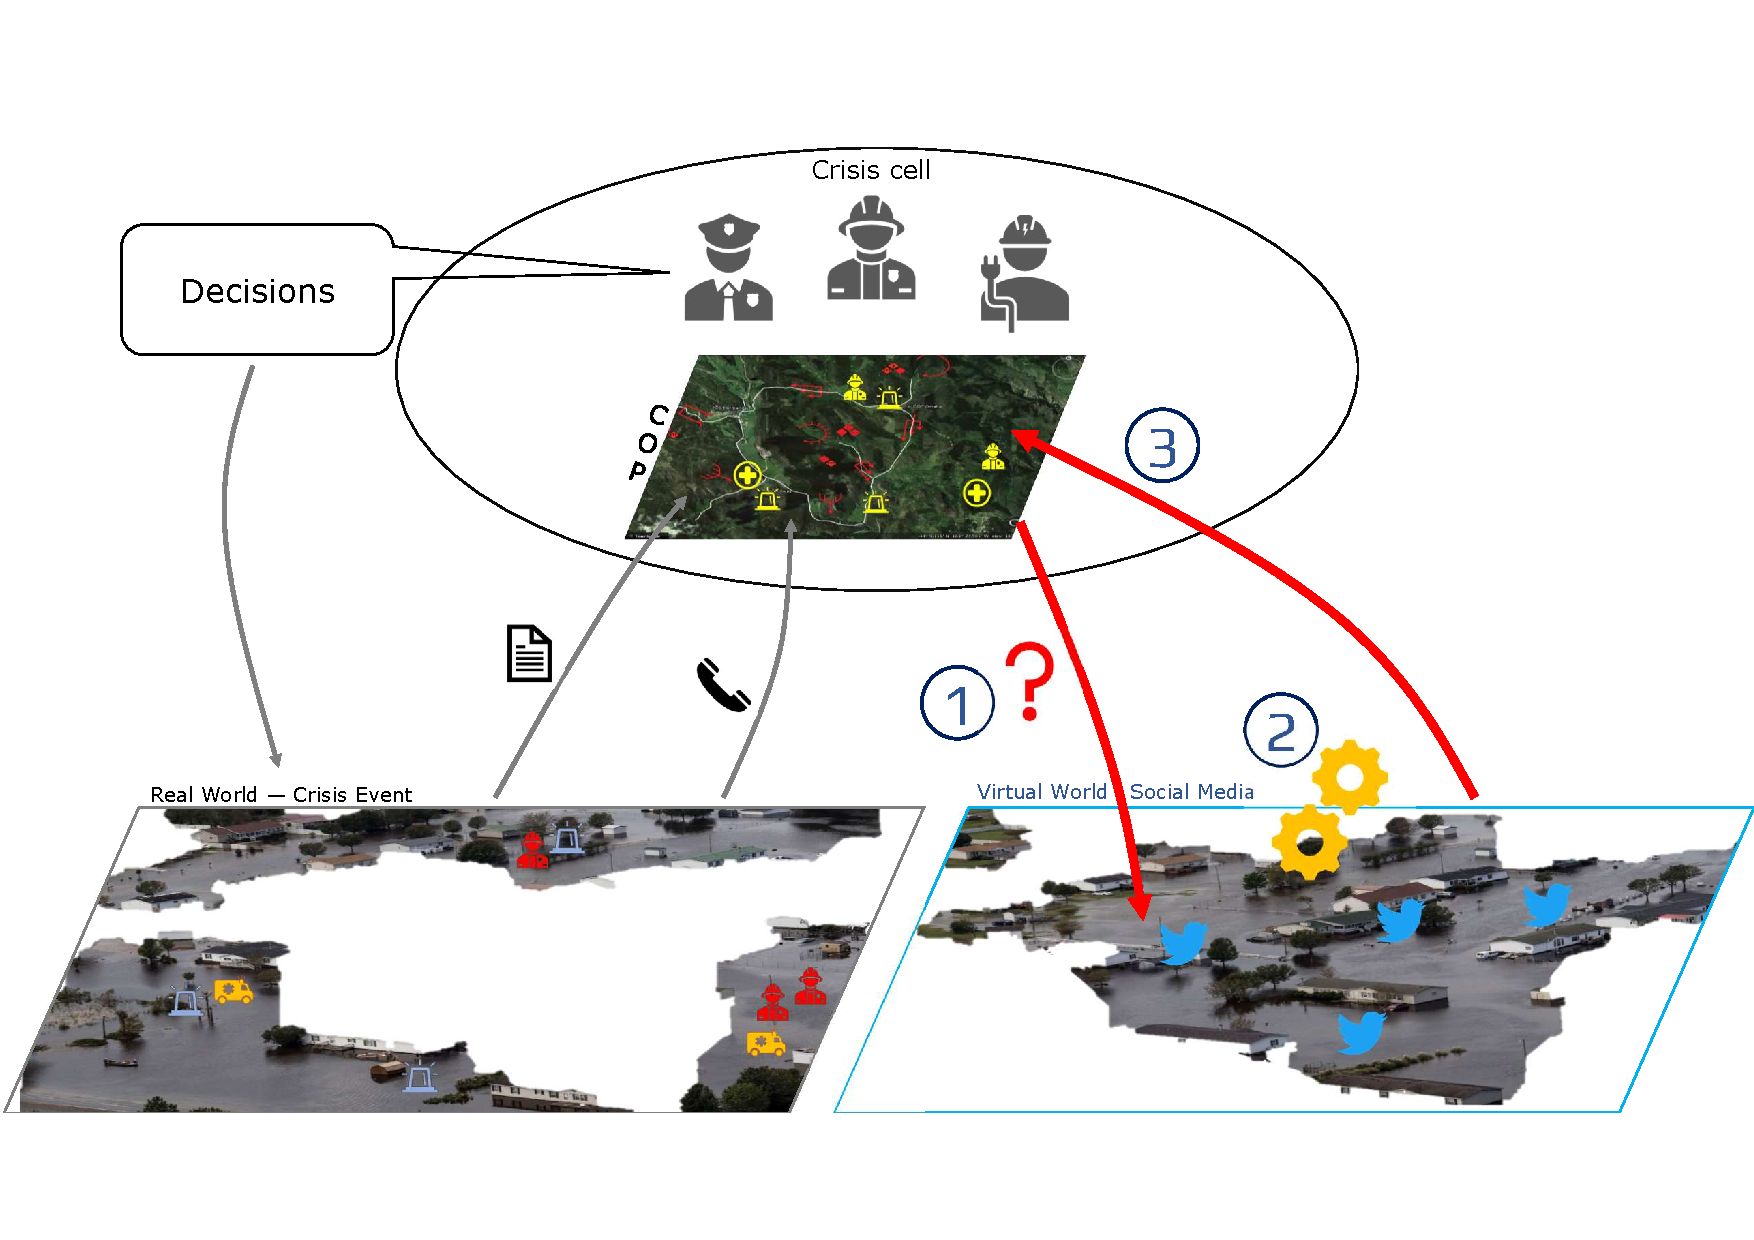
\includegraphics[width=\paperwidth,height=\paperheight,keepaspectratio]{figures/big-picture.pdf}
        \caption{Big picture of the manuscript.}
        \label{context:big-picture}
    \end{figure}
\end{landscape}

The next chapter, Chapter 2, is a literature review that explores the scope of each research question.
Chapters 3 to 5 are the contributions associated with each research question.

\begin{itemize}
    \item Chapter 3 narrows the scope of the information system designed by identifying its users and their information needs from an operational point of view.
    \item Chapter 4 describes an algorithm to identify the information needed, while maintaining the user in the information extraction process.
    \item Chapter 5 embeds all the previous contributions in a software architecture for a crisis information system, allowing to structure and build further information.
\end{itemize}

The final chapter, chapter 6, provide conclusion and discussions about this work.

%%% Local Variables:
%%% mode: latex
%%% TeX-master: "../ma-these"
%%% End:
